\section{Introduction}   \label{chap:introduction}

% > Goals:
% Hook
% What defines a real time system?
% What's an example of a real-time system?
% Where did RTS come from?
% What do they look like now?
% Why do we care about studying them?
\subsection{Logical and Temporal Correctness}
In 2018, an estimated 6.7 million car accidents in the US were reported - over 12 car accidents per minute \cite{noauthor_traffic_nodate}.
In vehicles sold in the US since 1998, an Electronic Control Unit (ECU) in the vehicle is responsible for determining if airbags should be deployed \cite{noauthor_airbags_nodate}.
The ECU uses wheel speed sensors, accelerometers, and Inertial Measurement Units (IMUs), to identify acceleration or vehicle speed sufficient to warrant deploying airbags. 
If needed, airbags are deployed in under 50 milliseconds \cite{amyleectrdotgov_air_2016}.
Since inception, the system of ECUs, sensors, and airbags have saved over 50,000 lives from car accidents and reduced the chance of fatality to drivers and front seat passangers by nearly 30\% \cite{noauthor_airbags_nodate}.
In this system, the improper calculation of acceleration or vehicle speed could result in deploying an airbag unnecessarily or worse - not deploying during a severe crash.
Even if the calculation is correct, however, deploying the airbag too late (after the driver or passenger have collided with the steering wheel or dashboard) could result in fatalities.
Airbag systems demonstrate the need for two types of correctness: logical and temporal.
The computation performed by the ECU must produce the correct signal to fire (or not fire) the airbags (logical correctness) \textbf{and} must produce the correct signal fast enough to save the occupants (temporal correctness).
Failure to guarantee either can result in death.
These systems, where logical and temporal correctness must be guaranteed to avoid catastrophe, are known as Real-Time Systems.

\begin{figure}
    \centering
    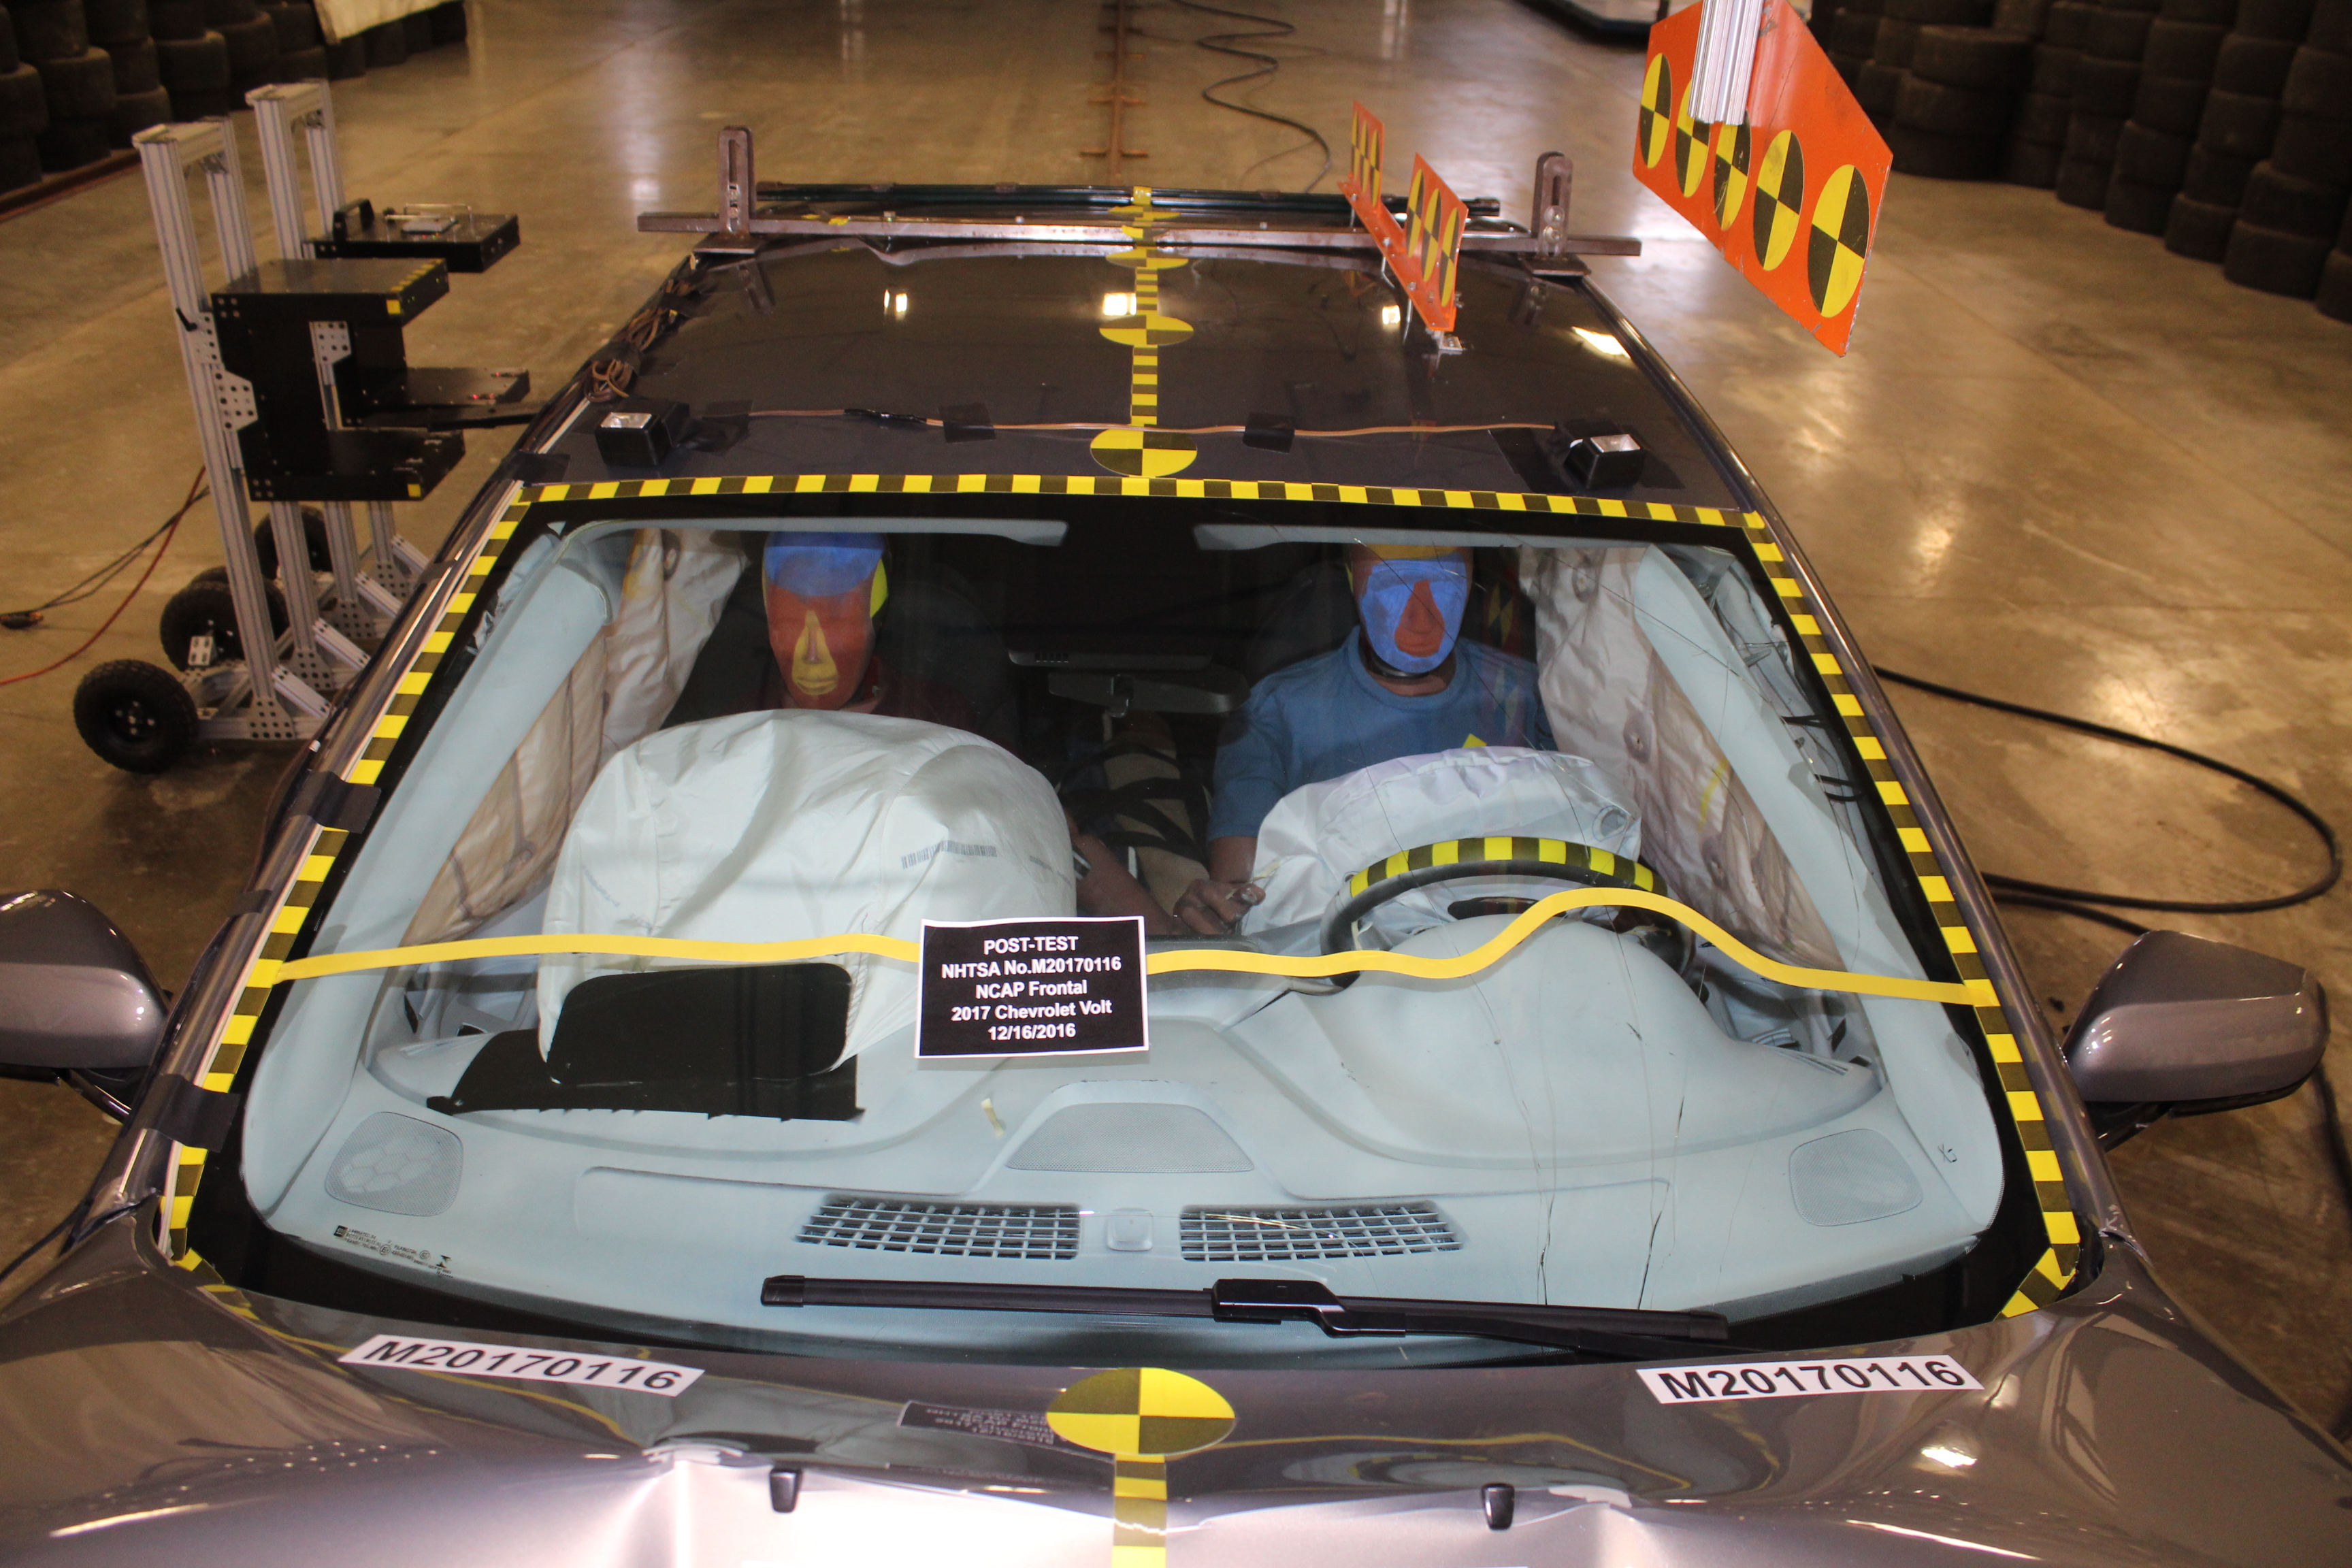
\includegraphics[width=0.75\linewidth]{fig/chevyVoltPostCrashTestDummies.jpg}
    \caption{Airbag Deployment in a Crash Test} Two crash test dummies sit in a 2017 Chevrolet Volt after a frontal crash.
    The airbag deployment in the Chevrolet Volt is controlled by its Air Bag Control Module \cite{noauthor_2014-2018_nodate}.
    The airbag deployment system is an example of a real-time system.

    Picture Credit: National Highway Transportation Safety Administration \cite{noauthor_nhtsa_nodate}.
    \label{fig:whirlwindComputer}
\end{figure}

% Introduce growing need for research that combines RTS and Control.
\subsection{What is a Real-Time System?}

In general, real-time systems are systems in which the utility of a computation depends on logical correctness of the result and timeliness of the computation CITE.
As illustrated by the airbag example, real-time systems are often present in safety-critical applications where incorrect or untimely operation leads to catastrophe.
% Example systems include TODO 

Consider, now, that accident detection and airbag deployment is not a calculation the ECU performs once but is calculated repeatedly.
This repeated calculation over time is referred to as a \textit{task}.
Note, formal definitions will be provided in Chapter \ref{chap:systemModel}.
Furthermore, the ECU may be responsible for more than airbag deployment - that is, the ECU may have more than one task to execute.
For each task on the ECU, some computation must be performed (fuel injection, spark ignition timing, throttle position sensing, wheel speed sensing, anti-lock braking, or traction control, for example).
Through code analysis, the time required to perform each task's computation can be upper bounded to give a \textit{Worst-Case Execution Time} (WCET).
Each task must also be executed at some particular frequency, known as a \textit{period}.
And each tasks' computed results must be known by some particular \textit{deadline}.
This combination of a task's WCET, period, and deadline is used to calculate \textit{demand} - the amount of processor time a task needs over time to guarantee calculations are completed before their respective deadlines.
This process of calculating demand is known as \textit{demand characterization}.
The study of real-time systems, therefore, involves characterizing the demand of some set of tasks, each with their own WCET, period, and deadline, to determine if a \textit{schedule}can be made for executing the tasks on a set of processors such that all computations are completed before their respective deadlines.
The analysis described above, called \textit{schedulability}, is one kind of analysis performed on real-time systems to guarantee logical and temporal correctness.
To better understand how real-time systems came to be, we now look toward the end of World War II.


% Consider, for example, the Electronic Control Unit (ECU) in a vehicle responsible for deploying airbags in the event of a crash \cite{hartl_airbag_1990}.
% An airbag ECU is an on-board computer that must correctly calculate acceleration from the vehicle's accelerometers or Inertial Measurement Units (IMUs) to identify rapid acceleration associated with an automobile crash.
% Failure to correctly calculate acceleration could result in airbag deployment when there is no need (possibly causing a crash) or worse: no airbag deployment when there is, in fact, a crash resulting in the injury or death of the driver (and/or other occupants).
% Suppose, however, that the ECU correctly determines when the airbags must deploy.
% If the ECU's acceleration and accident calculation takes too long (say, longer than the time required for the driver to collide with the steering column), deploying the airbag will be useless at best as the driver has already been injured or killed.
% The ECU responsible for deploying airbags, the sensors the ECU relies on, and even the airbag mechanisms themselves are all part of a real-time system in which logical and temporal correctness are required.

\subsection{The Rise of Real-Time Systems}

% Summary: Real-time systems are the follow up to real-time simulations. Post WWII simulations gave rise to real-time simulation. Managing telecommunications required real-time system modeling - the need for timely switching and routing of telephone signals to requested destination numbers. Eventually real-time systems were applied to industrial process control - the earliest of which was isomerization of butane in the chemical sector. In short, real-time systems began as a natural consequence of three things: simulating real-world control systems for military aircraft, serving user requests for telecommunications, and executing control of chemical process control.

The need for real-time systems began in 1944, at the close of World War II, when the US Navy initiated the development of Project Whirlwind, arguably the first American Real-Time System \cite{laplante_historical_1995}.
Driven by the need for pilots, Project Whirlwind, shown in Figure \ref{fig:whirlwindComputer}, aimed to develop a real-time flight control simulator \cite{forrester_whirlwind_1990}.
The project resulted in the first real-time computer, the Whirlwind Computer, which 
From the late 1940s to the 1950s, the Whirlwind Computer evolved into the Semi-Automatic Ground Environment (SAGE) air-defense system - a collection of radar stations. \cite{noauthor_tales_nodate}.
In the late 1950s, SAGE systems were installed by Canada and the United States as a joint effort under the North American Air Defense Command (now known as NORAD) to defend North American airspace on the verge of the Cold War\cite{lacomia_brief_nodate}.
In the 1950s, Bell Lab's engineers, recognizing the importance of timely switching and routing of phone calls, began treating telecom switching computers as real-time systems \cite{joel_communication_1957}.
As early as 1959, real-time systems were also applied to industrial control processes such as the isomerization of butane \cite{harrison_evolution_1981-1,stout_computer_1959}.
In each setting, real-time systems meet the need for correct computation in a timely manner to avoid otherwise catastrophic outcomes: lapse in air-defense, overloading of the telecommunications network and uncontrolled chemical reaction.

\begin{figure}
    \centering
    \includegraphics[width=0.75\linewidth]{fig/whirlwindComputer.JPG}
    \caption{Whirlwind} Segments of the Whirlwind Computer in the Museum of Science, Boston, Massachusetts, USA.
    Credit: 
    \label{fig:whirlwindComputer}
\end{figure}

\subsection{Modern Real-Time Systems and Why we Study Them}

% Summary: Modern RTS are now found in the same areas they began: aircraft, simulators, telecommunications, and industrial processes and have extended into more spaces.
% Real-time systems are found in autonomous (and non-autonomous vehicles), passenger aircraft, spacecraft, medical devices, and critical infrastructure.
% Modern RTS are not only concerned with safely executing control systems but also with reducing the Size, Weight and Power (SWaP) of devices.
% Modern RTS are also becoming more integrated with real-world dynamics by introducing .
% With the advent of CPS, RTS and Control Systems are further integrated.
% Modern RTS are not only converned with scheduling but also with SWaP.

Modern real-time systems are found in the same areas where they began: passenger and military aircraft, telecommunications, and chemical process control.
Real-time systems have also extended into autonomous (and non-autonomous) vehicles, spacecraft \cite{vavra_real-time_2018}, medical devices \cite{jiang_real-time_2010}, and critical infrastructure like dams, power stations, and water treatment plants.
Where a microcontroller can be found, so can a real-time system.
With ever smaller transistors, microcontrollers, and printed circuit boards, computing and control hardware is proliferating rapidly and becoming more intertwined with physical systems.
These systems where physical dynamics, hardware, and software are so closely integrated are known as Cyber-Physical Systems (CPS).
% CPSs are the foundation of "smart" infrastructure such as smart grids and smart homes and other connected dev
%given rise to new concepts like the Internet of Things, Cloud Computing, Edge Computing, and Cyber-Physical Systems.
The advent of CPSs has thus brought real-time systems and control systems closer together.
This close integration has magnifying the impact of advances in electronics and controls on real-time computing and vice versa.
% For example, effective real-time analysis can provide bounds on minimum required processor speed, helping system designers reduce the Size, Weight, and Power (SWaP) of their systems.

\subsection{Research Need}
% Summary: Growing number of devices, desire to lower SWaP, desire to integrate closely with physical world (CPS) require less pessimistic, more efficient, and more inclusive analysis.
The study of real-time systems is driven by the need for logical and temporal guarantees in increasingly complicated settings - in other words, predictable computing.
In real-time systems where multiple processors, multiple threads of execution, or tasks frequently change, guaranteeing correctness can be difficult and unintuitive.
Similarly, in systems where computational load is directly tied to system dynamics analysis can be nontrivial.
The integration of Real-Time Systems and control in Cyber-Physical Systems combined with the desire to lower SWaP creates a need for less pessimistic and more efficient demand characterization and schedulability analysis.
To illustrate why, consider the airbag deployment ECU example above.
If the real-time schedulability analysis is too pessimistic, a system may be declared unschedulable (and thus, unsafe) when, in fact, it is schedulable.
This pessimistic analysis may cause designers to purchase faster processors (or even more processors) than required.
In the best case, using a faster processor may only waste excess processor time, additional power required by the faster processor, and slightly increases the price of the system (for both the designer and the customer).
In the worst case, the system may need an additional processor entirely.
In a vehicle, this extra processor may mean an additional ECU complete with its own communication wiring, power wiring, enclosure, mounting brackets, and any space or weight consumed.
Clearly, the cost of the extra (possibly unnecessary) processor is more than just the processor itself.

Similarly, if the real-time schedulability analysis is too inefficient, providing real-time guarantees may be limited to offline settings where all tasks and computing hardware are known and fixed in advance.
This is problematic for real-world systems where hardware can fail (reducing the number of processors, for example), mistakes in modeling lead to jobs exceeding their WCET (meaning temporal correctness is no longer guaranteed), or when system workloads will change quickly with the addition and removal of tasks (changing the demand).
To adapt the schedule online, a real-time system must be able to recharacterize the demand and re-evaluate schedulability quickly.
Furthermore, in systems where online schedulability analysis is required the schedulability test itself reduces the processor availability for computing that tasks that are being scheduled!
In the pursuit of integrating real-time systems and control in Cyber-Physical Systems more realistic models of demand and more adaptive real-time systems require less pessimistic demand characterization and more efficient schedulability analysis. 

\begin{figure}
    \centering
    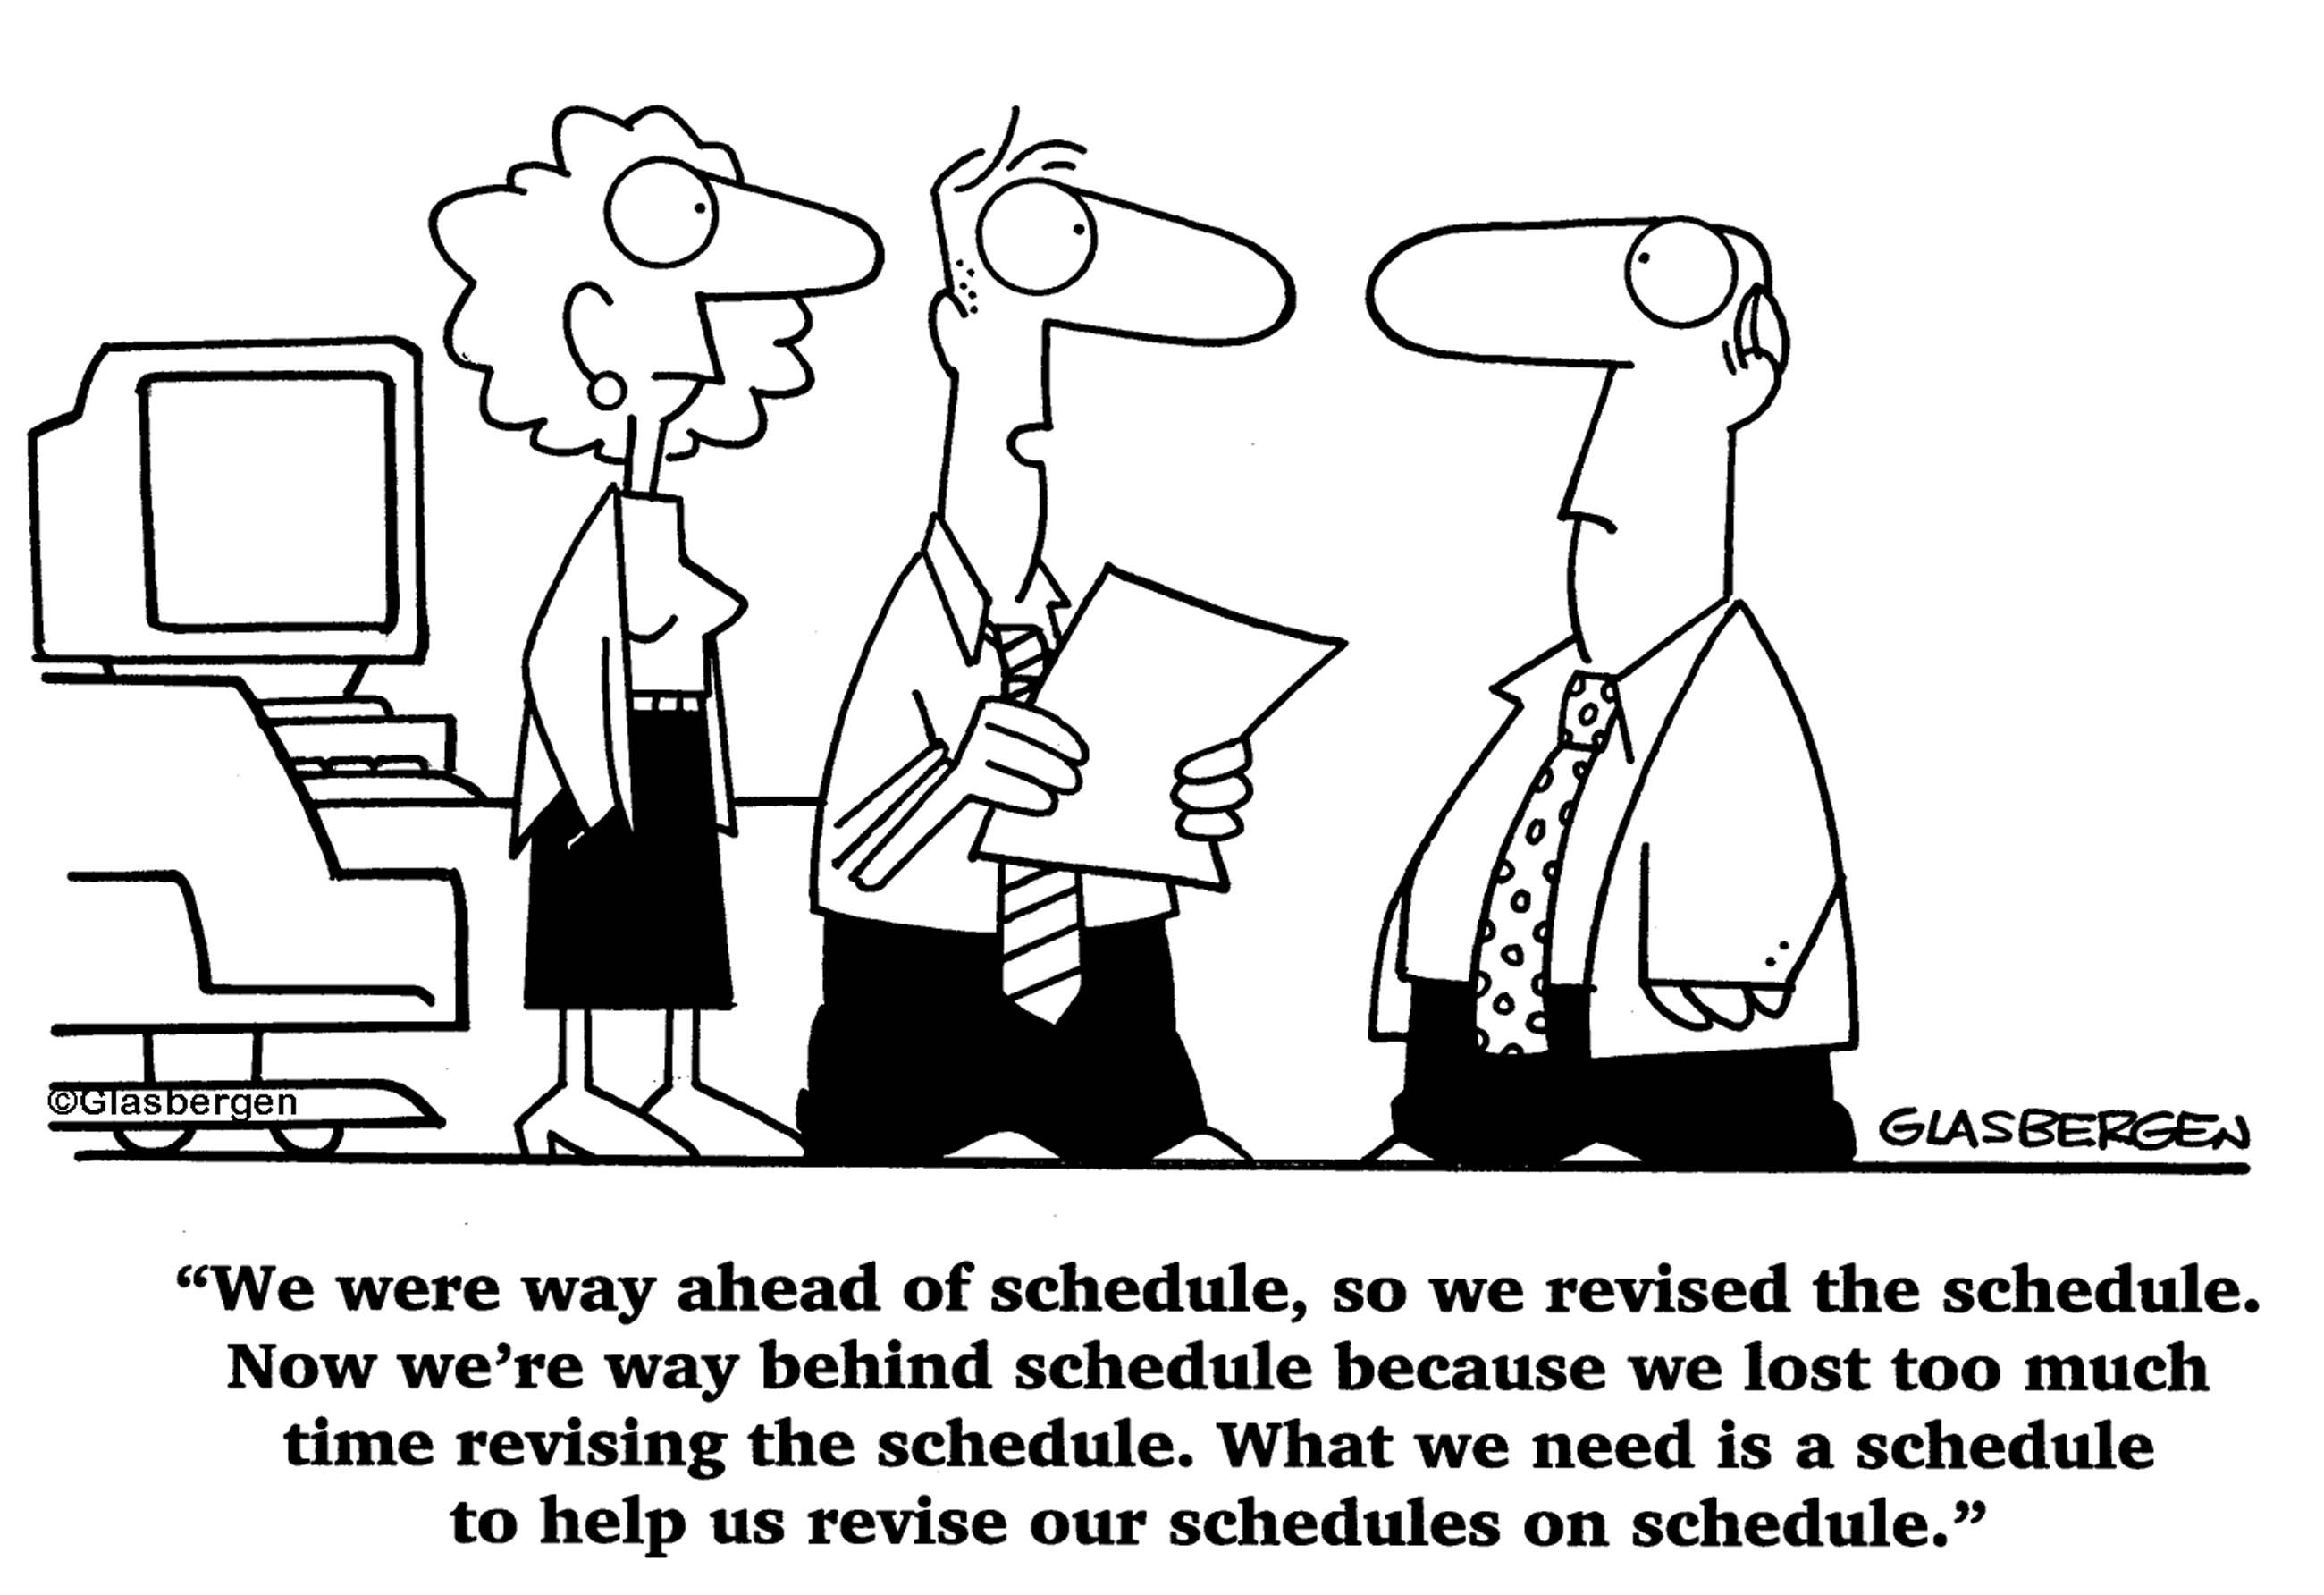
\includegraphics[width=0.7\linewidth]{fig/515.jpg}
    \caption{Scheduling Cartoon} A cartoon highlighting how scheduling itself takes time... sometimes too much time.

    Credit: Cartoon \copyright Glasbergen, used with special permission from \url{www.glasbergen.com}
\end{figure}

\subsection{Approach}
% > Incorporate physical dynamics of the systems whose workloads are being scheduled so that physical dynamics may be leveraged for more efficient demand characterization and schedulability analysis.
% Furthermore, incorporating physical dynamics will allow system designers to visualize tradeoffs between real-time metrics and physical system dynamics.
While the close integration of real-time systems with physical dynamics complicates analysis, it also presents an opportunity.
Physical systems have limitations set by physics.
In mechanical systems, these limitations may manifest as bounds on speed or acceleration.
In electrical systems, the limits may be on changes in current or voltage.
Thus, there is an opportunity to use the known properties of the physical system to mitigate the impact of the inherent complexity.
To address the need for less pessimistic and more efficient analysis in real-time cyber-physical systems, this work leverages limitations on physical system dynamics to characterize demand and perform schedulability analysis more efficiently while also enabling the codesign of hardware and software.
Specifically, this work aims to show how such limitations on physical dynamics can reduce the search space during demand characterization and schedulability analysis.
Similarly, this work aims to show how those same physical limitations and their relationship to real-time demand may be traded off with real-time system properties such as utilization and worst-case execution time.
This relationship allows system designers to directly relate physical system properties to system schedulability.

\subsection{Thesis}

In light of this opportunity, the main thesis of this work is:

"Incorporating physical dynamics into real-time system analysis can reduce pessimism and increase efficiency of demand characterization and schedulability analysis while enabling the codesign of real-time, cyber-physical systems." 

\subsection{Contributions}

The main contributions of this work are:
\begin{itemize}
    \item two inductor-based real-time software-based short-circuit detection methods,
    \item a hardware-software codesign approach for software-based short-circuit detection that demonstrates the tradeoff of processor utilization under EDF against inductor size (and thus board space consumed by circuitry),
    \item a demand characterization method for Adaptive Variable-Rate (AVR) tasks used in Internal Combustion Engines (ICEs) in which engine dynamics are used to limit the search space for the Demand Bound Function (DBF).
\end{itemize}

\subsection{Organization}

The remainder of this work is as follows:

\begin{enumerate}
    \item Chapter \ref{chap:relatedWork} summarizes the related work for each major contribution.
    \item Chapter \ref{chap:systemModel} provides the system model and terms common to each contribution.
    \item Chapter \ref{chap:codesign} covers the codesign of software-based short circuit protection systems.
    \item Chapter \ref{chap:scd} describes the demand characterization of AVR tasks in ICEs.
    \item Chapter \ref{chap:futureWork} discusses future work.
    \item Chapter \ref{chap:conclusion} summarizes and concludes this work.
    \item Chapter \ref{chap:publicationList} lists the publications which contributed to this work.
\end{enumerate}